\documentclass[a4j]{jarticle}

\usepackage{amsmath,amssymb,bm}
\usepackage{caption}
\usepackage{minitoc}
\usepackage{hhline}
\usepackage{algorithmic}
\usepackage{algorithm}
\usepackage{booktabs}
\usepackage[dvipdfmx]{graphicx} 
\usepackage[dvipdfmx, usenames]{color}
\usepackage{colortbl}
\usepackage{ascmac}
\usepackage{lscape}
\usepackage{url}
\usepackage{graphicx}
\usepackage{float}
\usepackage{siunitx}
\usepackage{subfig}
\usepackage{comment} 

\addtolength{\topmargin}{-2cm}
\addtolength{\textheight}{4cm}
\addtolength{\textwidth}{2cm}
\addtolength{\oddsidemargin}{-1cm}
\addtolength{\evensidemargin}{-1cm}


\begin{document}

\twocolumn[
\begin{center}
	{\Large タイコグラフィ法による大型X線ウォルターミラーの光学的評価}
\end{center}
\begin{center}
	{\Large Wave-optical evaluation of large-scale Wolter X-ray mirrors \vspace{2mm} \\ by ptychography measurement}
\end{center}

\begin{center}
	{\large 東京大学 ○渡辺貴史 竹尾陽子 山口豪太 三村秀和} \\
	{\large The University of Tokyo ○Watanabe Takafumi, Takeo Yoko, \\ Yamaguchi Gota, Mimura Hidekazu}
\end{center}
]

\section{序論}
天文分野において太陽の活動を観測することは非常に重要である。
2023年に打ち上げ予定のFOXSI4プロジェクトでは、太陽コロナの活発な領域において放射されるX線領域の電磁波を計測することで、これらの構造明らかにすることを1つの目標としている。
FOXSI4に搭載予定のWolter I型のミラーの解像分解能を向上させるためには、結像性能を悪化させる要因を特定し、その量を測定する装置が必要である。
測定装置は、ミラー内面を傷つけない非接触式であり、かつ素早く加工プロセスにフィードバックできる簡素なものが好ましい。
また、受光面積を大きくするため複数枚のWolterミラーをネスト構造にしたNested Wolterミラーに対しても適用可能な系であることが求められる。
これを満たす計測法として、形状誤差に起因する波面誤差から誤差量を逆算する波面計測法がある。
波面計測法では、1回の測定結果から様々な種類の形状誤差を統合的に計測することができ、非常に有用である。
Wolterミラーの集光波面は図\ref{fig:wolter_thinring}に示すように非常に細い輪帯状になっており、輪帯の幅(外円と内円の半径の差)は直径約 60 mm に対して\SI{363.3}{\micro \metre}となっている。
波面計測に求められる空間分解能が非常に高いものとなるため、波面計測法の中でも高分解能な測定が可能である位相回復法を採用する。

\begin{figure}[ht!]
\centering
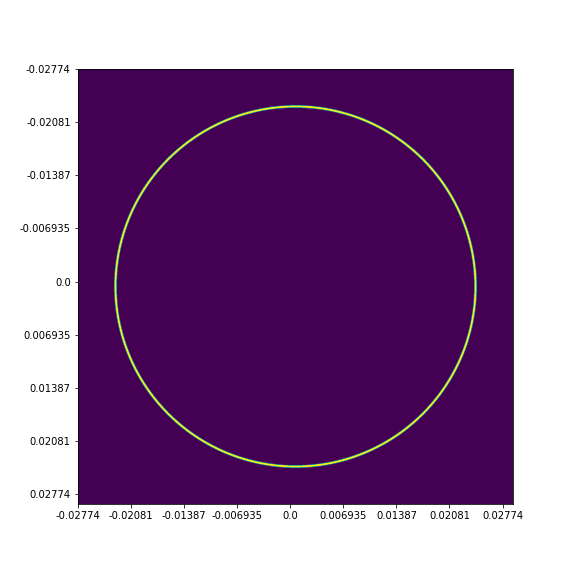
\includegraphics[width=7cm]{../thesis/chap1/figure/wolter_thinring.png}
\caption{Wolterミラー下流端面における集光波面}
\label{fig:wolter_thinring}
\end{figure}

\section{手法の検討}

位相回復法とは、測定対象の素子によって集光されたビームにオブジェクトを差し入れ、背後に現れる回折像の強度分布計測値から繰り返し計算によって位相情報を算出する方法である。
素子の最小サイズによる律速がないため、測定する際の配置を工夫することで非常に高い空間分解能が実現できる。
位相回復法の系として幾つかの種類が考えられる。
Wolterミラーが形成する集光ビームを測定対象とした場合、焦点面でオブジェクトを走査する方法ではミラー下流端面における空間分解能を十分確保するために必要な走査回数が数千回となってしまい、計測時間の観点から適切でない。

\subsection{下流端開口走査による冗長性}
\label{chap3_transverse_introduction}

オブジェクトを走査する位置を焦点面ではなく集光素子の開口直後とするTransverse Translation法がBradyらによって提案されている。\cite{Brady2009}
これは図\ref{fig:transverse_schematic}に示すように、焦点面を操作するタイコグラフィ法同様に穴の空いたピンホールオブジェクトを集光素子の開口で走査し、その回折像を下流側のカメラで撮影するという方法である。
この方法は、焦点面において1枚だけ強度分布を取得し位相回復計算を行う場合に比べ、ピンホールによりNAが低下し、メインローブの強度が下がるためダイナミックレンジの観点から有利である。

\begin{figure}[!ht]
\centering
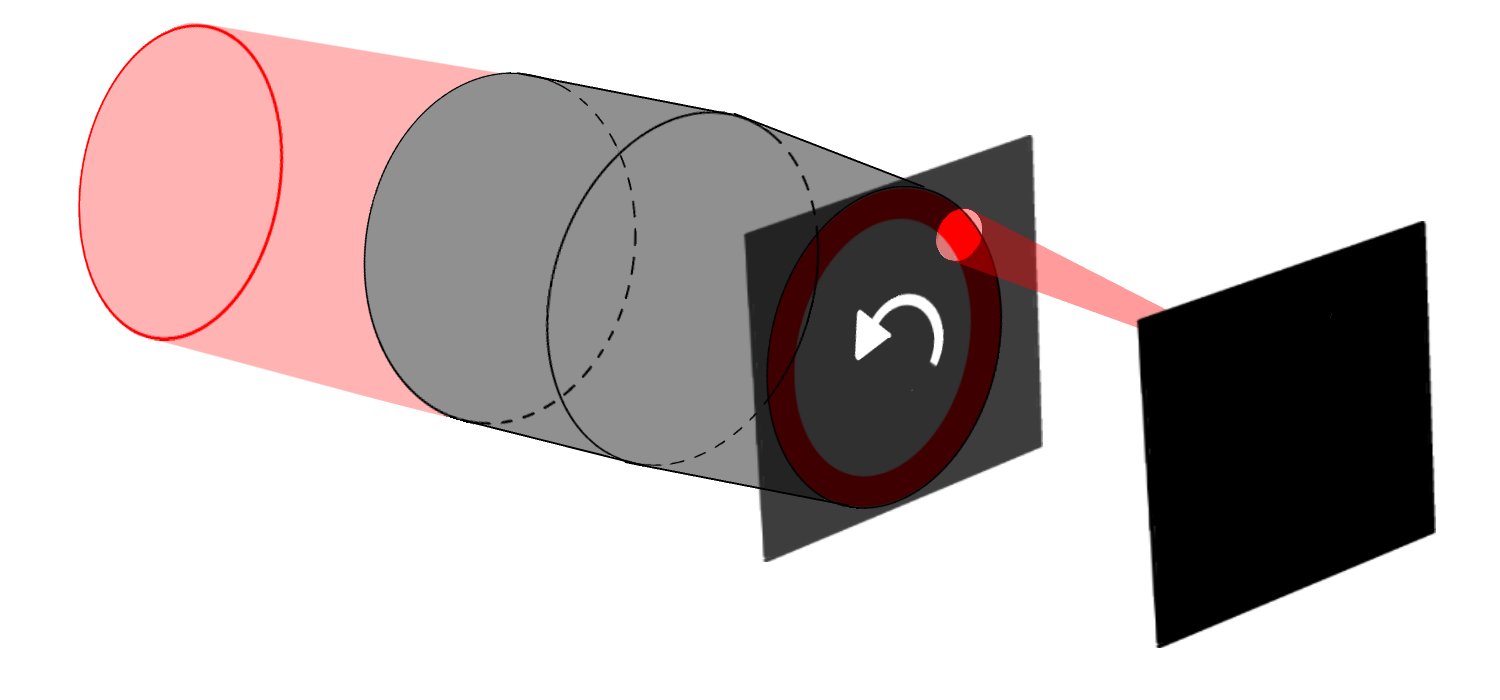
\includegraphics[width=6cm]{../thesis/chap3/figure/transverse_schematic.png}
\caption{下流端面走査による位相回復法の模式図}
\label{fig:transverse_schematic}
\end{figure}

\begin{figure}[!ht]
\centering
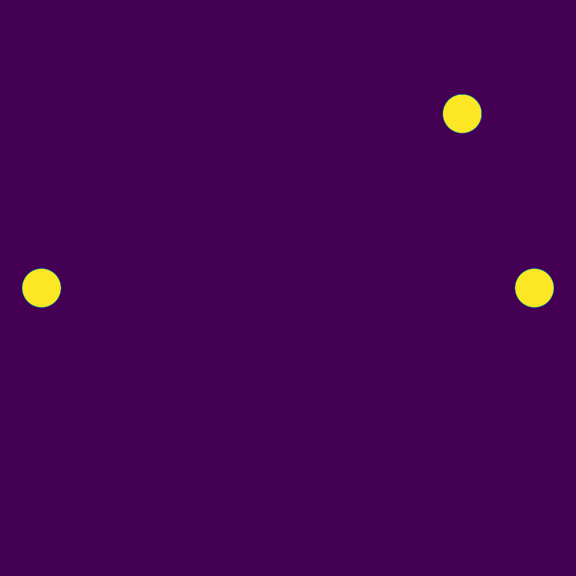
\includegraphics[width=5cm]{../thesis/chap3/figure/three_pinhole_mask.png}
\caption{3つ穴ピンホールの設計}
\label{fig:transverse_schematic}
\end{figure}

しかし、ビームの対称性から、ピンホールが1つでは位相回復計算が収束しない。
これを解決するため、穴を3つ不等間隔で開けたオブジェクトを用いて走査する方法を提案する。
シミュレーションによる検討から、不等間隔の3つ穴を持つピンホールオブジェクトによる位相回復計算が収束することを確認した。

\section{ミラー計測実験}

ミラーに合わせて実験装置を設計した。
ピンホールは自動回転ステージに取り付けられ、ミラー下流端直後に配置された。
ミラーの置き直しに対する再現性を高めるため、ミラーに合わせて把持機構を設計した。

\begin{figure}[!ht]
\centering
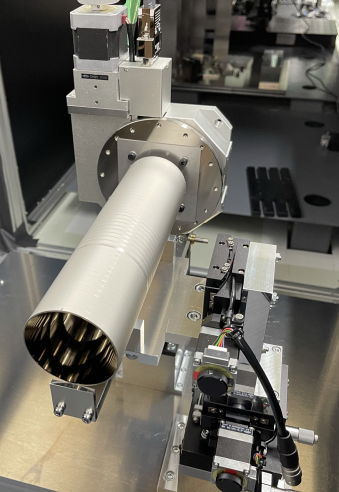
\includegraphics[width=4cm]{../thesis/chap5/figure/photo_mirror_pinhole.png}
\caption{ミラー測定実験系 写真}
\label{fig:photo_mirror_experiment_mirror_and_pinhole}
\end{figure}

2021年1月に三村グループによって作製されたWolterミラーに対して提案手法を適用し、測定実験を行った。

\begin{figure}[!ht]
\centering

\includegraphics[width=5cm]{../thesis/chap5/figure/reconstructed_phase_unwrapped.png}
\caption{回復された位相分布}
\label{fig:reconstructed_phase_unwrapped}
\end{figure}

\begin{figure}[!ht]
\centering
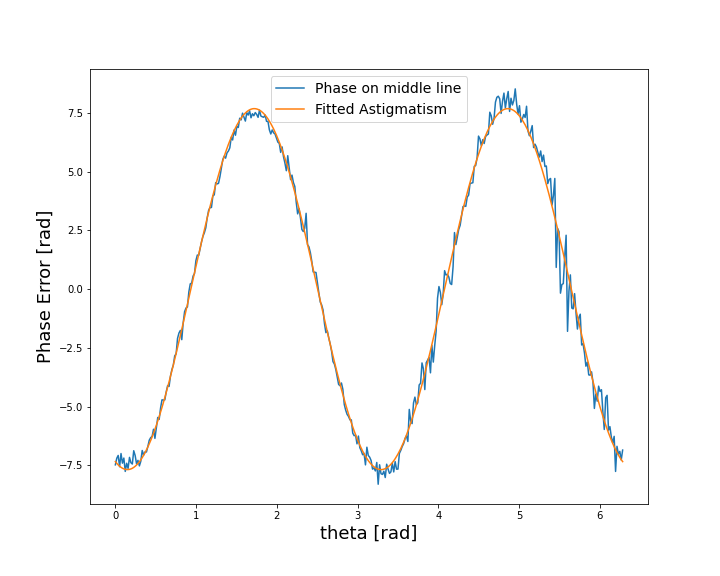
\includegraphics[width=5cm]{../thesis/chap5/figure/astigmatism_fitted.png}
\caption{フィッティングされた非点収差成分}
\label{fig:astigmatism_fitted}
\end{figure}

位相回復によって得られた強度および位相分布から焦点面での強度分布を再構成したところ、測定とは別に直接撮影された焦点面の強度分布と良く一致した。
このことから、位相回復計算の妥当性が確認できた。

さらに、位相分布について解析を行ったところ、図\ref{fig:astigmatism_fitted}に示すように周方向に非点収差成分に対応する誤差分布が確認された。
この非点収差成分をミラー形状における周方向誤差に換算するとp-v値で\SI{203}{\micro \metre}となった。
事前に行われた接触式の周方向プロファイル計測結果が示すp-v値は\SI{2}{\micro \metre}程度となっており、両者は矛盾する。
そこで、非点収差成分がミラーに起因するものであるかどうか確かめるため、ミラーを光軸方向周りに回転させて焦点面の強度分布の変化を観察したところ、強度分布はミラーに伴って回転することなく、同じ角度で留まった。
このことから、非点収差はミラーではなく上流光学系由来のものであると結論づけた。
理想的なレンズを用いた実験によって上流光学系を校正した上で、再度実験を行うことで、ミラーに起因する波面誤差が計測できると考えられる。

\section{結論}

求められるWolterミラー計測において、高空間分解能で撮影枚数の十分少ない計測法を提案し、シミュレーションによってその正当性を確認した。
ミラー測定実験については、上流光学系の再アラインメントおよび複数回の計測によるシステムエラーの除去を行う必要がある。
今後の展望として、ピンホールの穴サイズや穴の個数、配置する角度などの最適化による、安定性や撮影時間を改善が課題として挙げられる。
また、ネスト構造のWolterミラーにも同様の手法を適用し、計測実験を行うことが期待される。

\bibliography{references}
\bibliographystyle{siam}

\end{document}